\begin{samplecase}
{\bf Residual production cross section: ${}^{123}$Te(p,n): Global vs. adjusted calculation}\newline
This sample case shows the difference between a global TALYS calculation, with all nuclear model 
parameters at their default values, and a calculation with adjusted values for the most sensitive parameters 
in the 5-20 MeV energy range for (p,n) reactions. 
The (p,n) reaction is important since it often represents a good production route for medical isotopes.
The TASMAN code\cite{Koning2019} has been used to (a) determine the most important TALYS parameters from sensitivity profiles and 
(b) to optimize these parameters in a multi-dimensional parameter search. 
For the optimal result, the following parameters take on values within 10\% of their default values:
\begin{itemize}
\item radius of real volume potential $r_{V}$ for protons, see Eq. (\ref{par}),
\item radius of imaginary surface potential $r_{D}$ for protons, see Eq. (\ref{par}),
\item radius of real volume potential $r_{V}$ for neutrons, see Eq. (\ref{par}),
\item single-particle state density parameter for the compound nucleus, see Eq. (\ref{gpignu}),
\item single-particle state density parameter for the residual (p,n) nucleus, see Eq. (\ref{gpignu}),
\item total level density parameter for the residual (p,n) nucleus, see Eq. (\ref{micro}).
\end{itemize}
which amounts to 3 OMP parameters, 2 pre-equilibrium parameters and 1 compound nucleus parameter.
It is also important to filter the experimental data set for obvious outliers: in the current case the data from 
Barall et al\cite{Barall1981} has been excluded from the optimization, while those of Mahunka et al\cite{Mahunka1996} and 
Scholten et al\cite{Scholten1989} have been included.
It is interesting to see that both the global and fitted TALYS calculation, as well as the JENDL-5.0 evaluation \cite{JENDL5} 
follow the Mahunka data in the rising part of the excitation function, regardless of the inclusion of the Scholten data in the 
optimization of the fitted TALYS result. The IAEA evaluation \cite{IAEAmed} generally comes from least-squares fitting by means of Pade approximations.

It turns out that the above 6 parameters can be used to get a good (p,n) fit for all nuclides for which experimental data exist. 
Similar sets of 3-7 sensitive parameters can be identified to automatically optimize other excitation functions such as 
(n,$\gamma$), the combination of the three correlated channels (n,n'), (n,2n) and (n,p), (n,$\alpha$), (n,f), ($\alpha$,n) 
etc. for all nucldies for which experimental data exist.
Of course, one should always remember that there are model limitations which make it impossible to reproduce the required 
shape of the experimental excitation function (assuming these represent reality), even if we allow the parameter values to 
move away quite far from the default values.

We use the following input file with optimized parameters,

\VerbatimInput{\samples p-Te123-pn-fit/org/talys.inp}

while for the global calculation we simply remove, or comment, all the adjusted parameters at the end of the input file.
The resulting files {\em rp053123.tot} are plotted
together with experimental data in Fig.~\ref{p-Te123-pn-fit}.

\end{samplecase}
\begin{figure}
\centering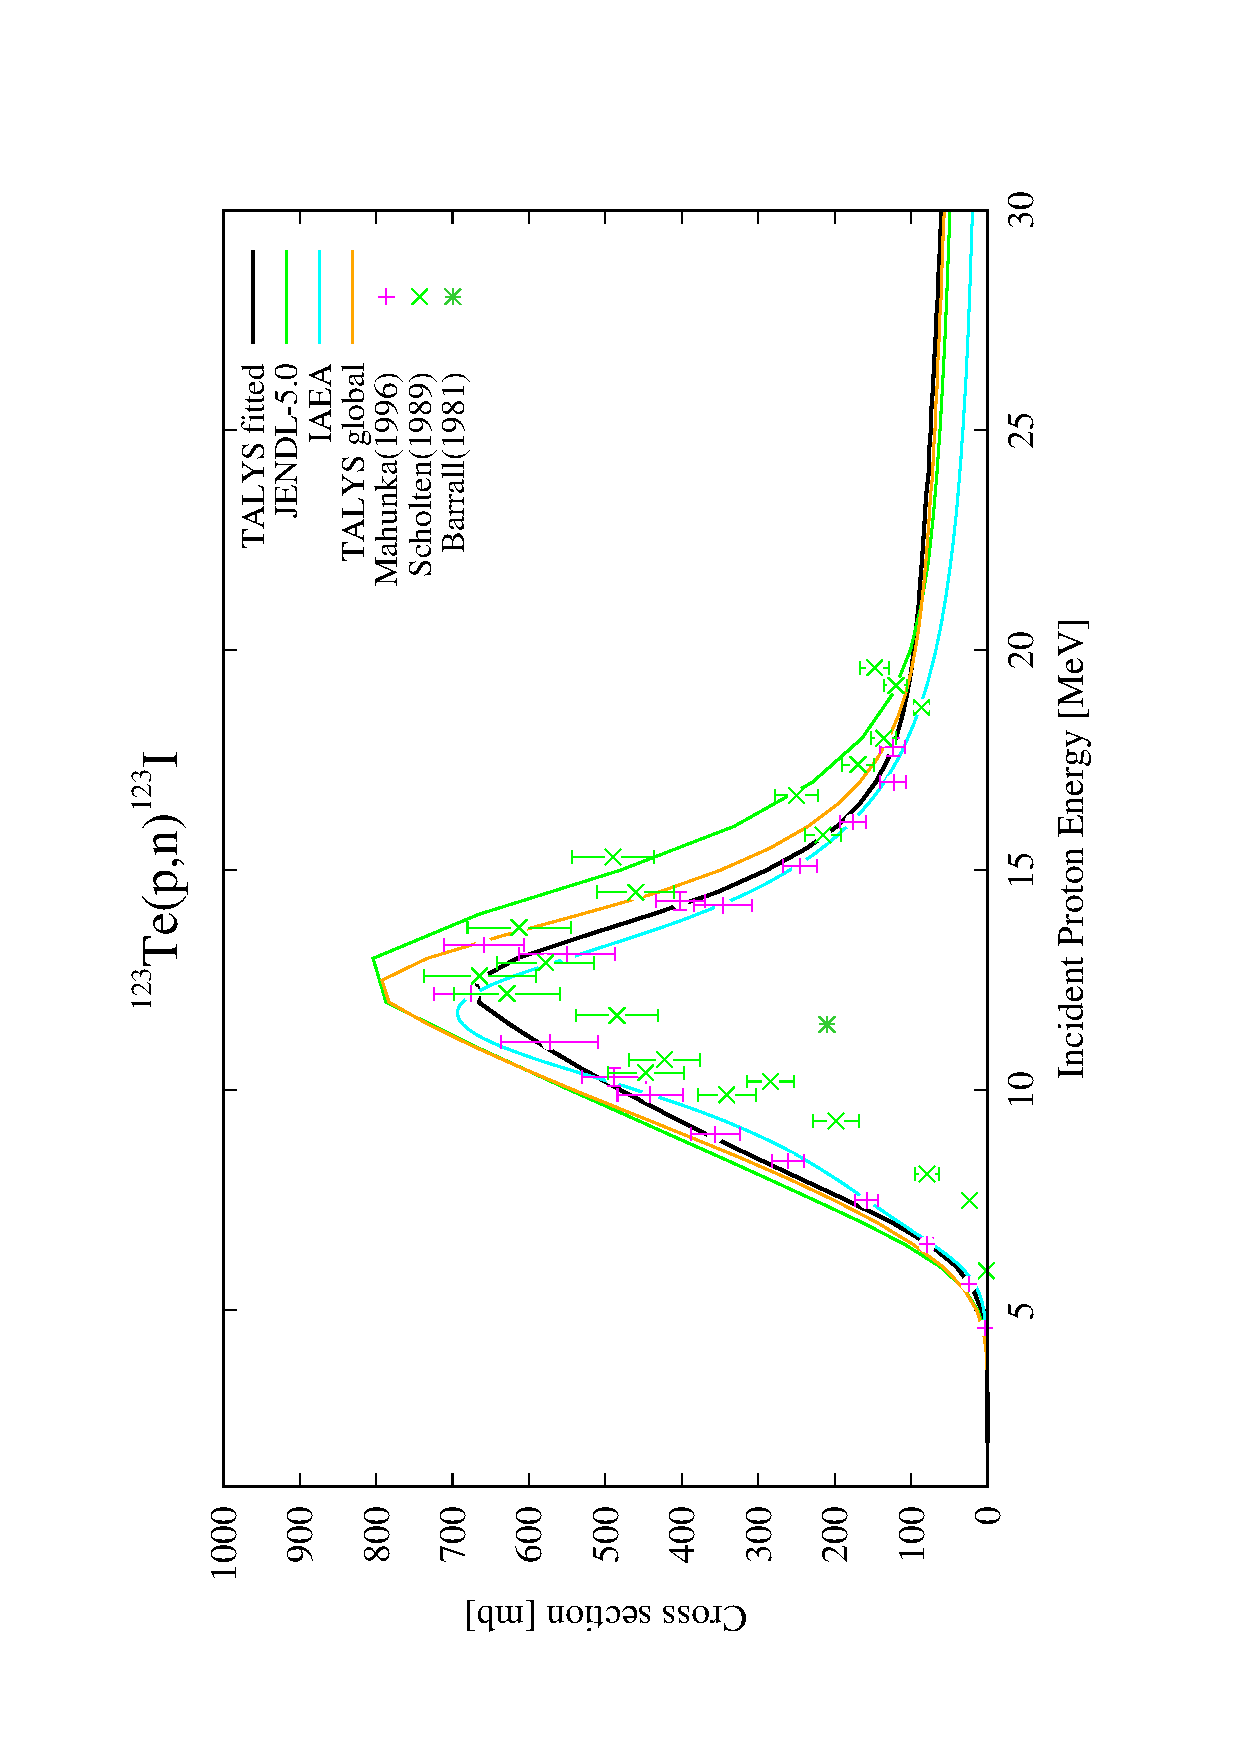
\includegraphics[scale=0.5,angle=270]{p-Te123-pn-fit}
\caption{Excitation function of ${}^{123}$Te(p,n) compared with existing nuclear data evaluations and
experimental data.}
\label{p-Te123-pn-fit}
\end{figure}
